% =============================================================================================
%  EpistemeGraph -- manuscript (IEEE conference format)
%  Every quantitative result is a macro defined in generated/results.tex, written by
%  scripts/analyze_results.py + scripts/export_paper_assets.py from the actual run artefacts.
%  Overleaf: upload paper/EpistemeGraph_overleaf.zip (New Project -> Upload Project) and press Recompile.
%  Local:    latexmk -pdf main.tex      (or pdflatex -> bibtex -> pdflatex x2)
% =============================================================================================
\documentclass[conference]{IEEEtran}
\IEEEoverridecommandlockouts

\usepackage[T1]{fontenc}
\usepackage[utf8]{inputenc}
\usepackage{cite}
\usepackage{amsmath,amssymb,amsthm,mathtools}
\usepackage{bm}
\usepackage{booktabs}
\usepackage{graphicx}
\usepackage{adjustbox}
\usepackage{xcolor}
\usepackage{algorithm}
\usepackage{algpseudocode}
\usepackage{microtype}
\usepackage[colorlinks=true,linkcolor=blue!50!black,citecolor=blue!50!black,urlcolor=blue!50!black]{hyperref}
\usepackage[capitalise,noabbrev]{cleveref}

\newtheorem{definition}{Definition}
\newtheorem{proposition}{Proposition}
\newtheorem{lemma}{Lemma}

\DeclareMathOperator{\logit}{logit}
\DeclareMathOperator{\spec}{spec}
\DeclareMathOperator*{\argmin}{arg\,min}
\newcommand{\R}{\mathbb{R}}
\newcommand{\E}{\mathbb{E}}
\newcommand{\SKGq}{S_{\mathrm{KG}}(q)}
\newcommand{\todo}[1]{\textcolor{red!70!black}{[#1]}}

% ---- results (auto-generated); the fallback keeps the source compilable before any run -----------
\IfFileExists{generated/results.tex}{% AUTO-GENERATED by scripts/export_paper_assets.py -- do not edit by hand
\newcommand{\SKG}{84.4}
\newcommand{\PhiProv}{86.8}
\newcommand{\PhiCov}{69.8}
\newcommand{\PhiTopo}{84.3}
\newcommand{\PhiCons}{99.5}
\newcommand{\NDocs}{3}
\newcommand{\NChunks}{76}
\newcommand{\NRawTriples}{613}
\newcommand{\NTriples}{375}
\newcommand{\NEntities}{313}
\newcommand{\NShared}{29}
\newcommand{\AcceptRate}{61.2}
\newcommand{\KGPrec}{53.0}
\newcommand{\KGPrecLo}{43.3}
\newcommand{\KGPrecHi}{62.5}
\newcommand{\KGPrecLenient}{85.0}
\newcommand{\KGAuditN}{100}
\newcommand{\KGAuditor}{claude-haiku-5-5}
\newcommand{\NItems}{400}
\newcommand{\NLabelled}{400}
\newcommand{\NTrain}{262}
\newcommand{\NCal}{65}
\newcommand{\NTest}{73}
\newcommand{\SupportedRate}{19.5}
\newcommand{\ExtentHal}{80.8}
\newcommand{\ExtentSup}{75.9}
\newcommand{\ExtentAUC}{0.511}
\newcommand{\Champion}{MonotoneHistGBM}
\newcommand{\TestAUC}{0.728}
\newcommand{\TestLL}{0.402}
\newcommand{\TestBrier}{0.123}
\newcommand{\TestECE}{0.054}
\newcommand{\TestAcc}{84.9}
\newcommand{\LLMAUC}{0.797}
\newcommand{\LLMECE}{0.324}
\newcommand{\Alpha}{0.10}
\newcommand{\Coverage}{97.3}
\newcommand{\CoverageSup}{92.3}
\newcommand{\CoverageHal}{98.3}
\newcommand{\AbstainRate}{76.7}
\newcommand{\SelAcc}{88.2}
\newcommand{\TauVer}{0.084}
\newcommand{\TauHal}{0.313}
\newcommand{\PoolBzero}{4.07}
\newcommand{\PoolBq}{0.98}
\newcommand{\PoolBkg}{-1.23}
\newcommand{\JudgeKappa}{--}
\newcommand{\JudgeN}{--}
\newcommand{\PrimaryJudge}{claude-sonnet-5-5}
\newcommand{\CrossJudge}{claude-haiku-5-5}
\newcommand{\CrossJudgeN}{100}
\newcommand{\CrossJudgeKappa}{0.35}
\newcommand{\CrossJudgeAgree}{80.0}
\newcommand{\TestAUCLo}{0.562}
\newcommand{\TestAUCHi}{0.870}
\newcommand{\LLMAUCLo}{0.612}
\newcommand{\LLMAUCHi}{0.927}
\newcommand{\DeltaLLM}{-0.069}
\newcommand{\PvalLLM}{0.492}
\newcommand{\DeltaText}{0.032}
\newcommand{\PvalText}{0.774}
\newcommand{\DeltaTopo}{0.010}
\newcommand{\PvalTopo}{0.797}
\newcommand{\KGAccLearned}{54.1}
\newcommand{\KGAccLo}{45.6}
\newcommand{\KGAccHi}{62.6}
\newcommand{\SensDefault}{0.8446}
\newcommand{\SensMaxDev}{0.0342}
\newcommand{\SensRange}{0.0557}
\newcommand{\AnswerModel}{claude-haiku-5-5}
\newcommand{\JudgeModel}{claude-sonnet-5-5}
\newcommand{\CVProtocol}{5x5 repeated stratified CV, n=400}
\newcommand{\CVAUC}{0.742}
\newcommand{\CVAUCsd}{0.052}
\newcommand{\CVAUCLo}{0.633}
\newcommand{\CVAUCHi}{0.780}
\newcommand{\CVAUCvthree}{0.737}
\newcommand{\CVAUCtext}{0.705}
\newcommand{\CVAUCllm}{0.591}
\newcommand{\CVAUClen}{0.628}
\newcommand{\CVECE}{0.090}
\newcommand{\CVECEllm}{0.342}
\newcommand{\CVPvthree}{0.588}
\newcommand{\CVPllm}{0.022}
\newcommand{\CVPtext}{0.876}
\newcommand{\CVPlen}{0.049}
\newcommand{\SevereAUC}{0.708}
\newcommand{\SevereLLM}{0.662}
\newcommand{\SevereN}{300}
\newcommand{\VthreeTestAUC}{0.671}
\newcommand{\VthreeChampion}{RandomForest}
\newcommand{\KappaUnsup}{0.48}
\newcommand{\KappaOrd}{0.41}
\newcommand{\AUCvsSecond}{0.714}
\newcommand{\AUCvsPrimarySame}{0.723}
\newcommand{\AUCagree}{0.756}
\newcommand{\NAgree}{80}
\newcommand{\LenAUC}{0.604}
\newcommand{\FPAccepted}{38.8}
\newcommand{\NPartial}{222}
\newcommand{\NUnsup}{100}
\newcommand{\NSup}{78}
\newcommand{\CostRun}{1.90}
\newcommand{\KappaFull}{0.57}
\newcommand{\AgreeFull}{87.2}
\newcommand{\ConsensusN}{349}
\newcommand{\ConsensusAUC}{0.762}
\newcommand{\ConsensusLLM}{0.571}
\newcommand{\ConsensusMatched}{305}
\newcommand{\GeminiName}{Gemini Pro (high reasoning)}
\newcommand{\GeminiSupp}{70.0}
\newcommand{\GeminiKappa}{0.17}
\newcommand{\GeminiAUC}{0.486}
\newcommand{\GeminiLLMAUC}{0.714}
\newcommand{\MajorityAUC}{0.727}
\newcommand{\MajorityLLMAUC}{0.650}
\newcommand{\NUnanimous}{32}
\newcommand{\ThirdJudgeSentence}{A third judge from a different model family (\texttt{Gemini Pro (high reasoning)}), given the three papers in full and blind to the other verdicts, labelled the same 100 answers; its binary agreement with the primary judge is $\kappa=0.17$ (raw agreement 49.0\%).}
\newcommand{\HumanJudgeSentence}{}
\newcommand{\HaikuLabelCVAUC}{0.736}
\newcommand{\HaikuLabelCVAUCllm}{0.548}
\newcommand{\HaikuLabelCVAUCvthree}{0.697}
\newcommand{\CatCrossLLM}{0.219}
\newcommand{\CatFPLLM}{0.709}
\newcommand{\HKvsSonnet}{0.797}
\newcommand{\HKvsHaiku}{0.722}
\newcommand{\HaikuLabelKappa}{0.35}
\newcommand{\MatchN}{330}
\newcommand{\MatchTotal}{400}
\newcommand{\MatchBase}{322}
\newcommand{\BalAcc}{62.9}
\newcommand{\Committed}{137}
\newcommand{\CommittedCorrect}{114}
\newcommand{\KGPrecLenientLo}{76.7}
\newcommand{\KGPrecLenientHi}{90.7}
\newcommand{\KGNIncorrect}{15}
\newcommand{\KGNPartial}{32}
\newcommand{\CVCovTen}{94.2}
\newcommand{\CVAbsTen}{65.8}
\newcommand{\CVSelTen}{83.0}
\newcommand{\CVAbsTwenty}{48.8}
\newcommand{\CVSelTwenty}{83.1}
\newcommand{\PoolLRTp}{0.040}
\newcommand{\PoolLRTchi}{4.22}
\newcommand{\PoolKGused}{kept}
\newcommand{\CatBorderLLM}{0.341}
\newcommand{\CatBorderLen}{0.752}
\newcommand{\CatBorderVfour}{0.685}
\newcommand{\CatCrossVfour}{0.539}
\newcommand{\CatCrossVthree}{0.664}
\newcommand{\CatFactLLM}{0.759}
\newcommand{\CatFactVfour}{0.695}
\newcommand{\CatFPVfour}{0.776}
\newcommand{\PoolCVwith}{0.4494}
\newcommand{\PoolCVwithout}{0.4506}
\newcommand{\TestAUCq}{0.746}
\newcommand{\AUCvsSecondLLM}{0.395}
\newcommand{\OrdAUC}{0.739}
\newcommand{\BinAUC}{0.734}

\newcommand{\TableCv}{%
\begin{table}[t]\centering\footnotesize
\caption{Repeated cross-validation over all labelled answers (\CVProtocol). Pooled out-of-fold AUROC, mean $\pm$ s.d. over folds, 95\% bootstrap CI and ECE of one repetition, and the paired DeLong $p$-value against EpistemeGraph v4.}\label{tab:cv}
\begin{adjustbox}{max width=\columnwidth}\begin{tabular}{lccccc}\toprule
Detector & AUROC & fold mean $\pm$ s.d. & 95\% CI & ECE & $p$ (DeLong) \\ \midrule
\textbf{EpistemeGraph} & 0.742 & 0.741 $\pm$ 0.052 & [0.633, 0.780] & 0.090 & -- \\
Same learner, 13 answer features & 0.737 & 0.741 $\pm$ 0.066 & [0.659, 0.792] & 0.079 & $0.588$ \\
Text-only NLI checker & 0.705 & 0.708 $\pm$ 0.068 & [0.640, 0.776] & 0.027 & $0.876$ \\
LLM verbalised confidence & 0.591 & 0.591 $\pm$ 0.076 & [0.504, 0.677] & 0.342 & $0.022$ \\
Answer length & 0.628 & 0.634 $\pm$ 0.078 & [0.551, 0.702] & 0.042 & $0.049$ \\
\bottomrule\end{tabular}\end{adjustbox}
\end{table}}

\newcommand{\TableConformal}{%
\begin{table}[t]\centering\footnotesize
\caption{Risk--abstention trade-off of the Mondrian cross-conformal decision over all labelled answers (out-of-fold scores, 5-fold calibration).}\label{tab:conformal}
\begin{adjustbox}{max width=\columnwidth}\begin{tabular}{cccccc}\toprule
$\alpha$ & Coverage & Cov.\ sup. & Cov.\ hal. & Abstain & Sel.\ acc. \\ \midrule
0.05 & 95.8 & 96.2 & 95.7 & 82.2 & 76.5 \\
0.10 & 94.2 & 91.2 & 95.0 & 65.8 & 83.0 \\
0.15 & 93.2 & 86.2 & 95.0 & 60.5 & 82.7 \\
0.20 & 91.5 & 77.3 & 95.0 & 48.8 & 83.1 \\
0.25 & 91.2 & 76.1 & 95.0 & 41.0 & 85.4 \\
0.30 & 90.5 & 72.2 & 95.0 & 38.5 & 84.8 \\
\bottomrule\end{tabular}\end{adjustbox}
\end{table}}

\newcommand{\TableClaimimp}{%
\begin{table}[t]\centering\footnotesize
\caption{Grouped permutation importance of the pooled claim statistics (mean, min, max of one claim feature permuted jointly; increase in test log-loss).}\label{tab:claimimp}
\begin{adjustbox}{max width=\columnwidth}\begin{tabular}{lcc}\toprule
Claim feature & $\Delta$ log-loss & s.d. \\ \midrule
NLI contradiction & 0.0097 & 0.0155 \\
NLI entailment & 0.0079 & 0.0063 \\
Out-of-corpus rate & 0.0053 & 0.0031 \\
Grafted-edge curvature & 0.0053 & 0.0044 \\
Provenance strength & 0.0044 & 0.0048 \\
Evidence similarity & 0.0019 & 0.0024 \\
Sheaf residual & 0.0017 & 0.0033 \\
Two-hop KG path & 0.0015 & 0.0007 \\
Speculative polarity & 0.0013 & 0.0012 \\
Entity alignment & 0.0012 & 0.0017 \\
Refuted polarity & 0.0002 & 0.0006 \\
Conflict flag & 0.0000 & 0.0000 \\
Asserted polarity & -0.0013 & 0.0014 \\
Direct KG edge & -0.0017 & 0.0040 \\
NLI consistency & -0.0085 & 0.0061 \\
\bottomrule\end{tabular}\end{adjustbox}
\end{table}}

\newcommand{\TableLeaderboard}{%
\begin{table}[t]\centering\footnotesize
\caption{Ten-model tournament (nested 5$\times$3 CV on the training split, out-of-fold metrics). $^\star$ marks the champion, selected by log-loss.}\label{tab:leaderboard}
\begin{adjustbox}{max width=\columnwidth}\begin{tabular}{lcccc}\toprule
Model & Log-loss$\downarrow$ & AUROC$\uparrow$ & Brier$\downarrow$ & ECE$\downarrow$ \\ \midrule
Monotone gradient boosting$^\star$ & 0.373 & 0.809 & 0.117 & 0.062 \\
Gradient boosting & 0.376 & 0.807 & 0.116 & 0.041 \\
Stacking ensemble & 0.388 & 0.774 & 0.117 & 0.040 \\
Random forest & 0.397 & 0.768 & 0.121 & 0.069 \\
RBF-kernel SVM & 0.405 & 0.767 & 0.124 & 0.034 \\
Extra trees & 0.416 & 0.756 & 0.129 & 0.044 \\
Logistic regression & 0.418 & 0.720 & 0.127 & 0.037 \\
Attention MIL network & 0.495 & 0.562 & 0.149 & 0.051 \\
Multilayer perceptron & 0.573 & 0.438 & 0.189 & 0.175 \\
Attention ResNet & 0.621 & 0.632 & 0.209 & 0.221 \\
\bottomrule\end{tabular}\end{adjustbox}
\end{table}}

\newcommand{\TableAblation}{%
\begin{table}[t]\centering\footnotesize
\caption{Feature-family ablation (standardised logistic model, held-out test split; 95\% bootstrap CI).}\label{tab:ablation}
\begin{adjustbox}{max width=\columnwidth}\begin{tabular}{lcccc}\toprule
Feature set & AUROC & 95\% CI & Log-loss & ECE \\ \midrule
All inputs & 0.731 & [0.559, 0.867] & 0.450 & 0.111 \\
13 answer features only & 0.763 & [0.608, 0.888] & 0.403 & 0.119 \\
Pooled claims only & 0.638 & [0.444, 0.811] & 0.470 & 0.128 \\
Topological only & 0.631 & [0.439, 0.796] & 0.446 & 0.095 \\
Evidential only & 0.637 & [0.415, 0.830] & 0.455 & 0.112 \\
Model signals only & 0.758 & [0.583, 0.920] & 0.395 & 0.120 \\
Text NLI only & 0.696 & [0.511, 0.854] & 0.426 & 0.078 \\
Graph only & 0.650 & [0.445, 0.814] & 0.449 & 0.103 \\
Without topological & 0.721 & [0.530, 0.886] & 0.418 & 0.042 \\
Without model signals & 0.651 & [0.469, 0.826] & 0.481 & 0.101 \\
\bottomrule\end{tabular}\end{adjustbox}
\end{table}}

\newcommand{\TableSens}{%
\begin{table}[t]\centering\footnotesize
\caption{Phase 1 robustness: every design constant perturbed one at a time and the pipeline re-run on the cached extractions (no API calls).}\label{tab:sens}
\begin{adjustbox}{max width=\columnwidth}\begin{tabular}{lccccccc}\toprule
Constant & Value & $S_{\mathrm{KG}}$ & $\Phi_{\mathrm{prov}}$ & $\Phi_{\mathrm{cov}}$ & $\Phi_{\mathrm{topo}}$ & Triples & Entities \\ \midrule
all defaults & -- & 0.8446 & 0.869 & 0.698 & 0.843 & 375 & 313 \\
verbatim quote-match ratio & 0.75 & 0.8446 & 0.869 & 0.698 & 0.843 & 375 & 313 \\
verbatim quote-match ratio & 0.9 & 0.8446 & 0.869 & 0.698 & 0.843 & 375 & 313 \\
entity support in the quote & 0.75 & 0.8788 & 0.869 & 0.771 & 0.897 & 552 & 408 \\
entity support in the quote & 0.95 & 0.8446 & 0.869 & 0.698 & 0.843 & 375 & 313 \\
coverage normaliser tau & 0.5 & 0.8649 & 0.869 & 0.768 & 0.843 & 375 & 313 \\
coverage normaliser tau & 0.7 & 0.8231 & 0.869 & 0.630 & 0.843 & 375 & 313 \\
min. extractor confidence & 0.3 & 0.8443 & 0.868 & 0.698 & 0.843 & 375 & 313 \\
min. extractor confidence & 0.7 & 0.8453 & 0.871 & 0.697 & 0.845 & 374 & 311 \\
entity-merge cosine & 0.8 & 0.8486 & 0.869 & 0.697 & 0.861 & 374 & 295 \\
entity-merge cosine & 0.9 & 0.8454 & 0.869 & 0.701 & 0.842 & 381 & 324 \\
\bottomrule\end{tabular}\end{adjustbox}
\end{table}}

\newcommand{\TableTripleweights}{%
\begin{table}[t]\centering\footnotesize
\caption{Learned weights of the triple-correctness model used by the model-assisted KG-accuracy estimator (standardised logistic coefficients).}\label{tab:tripleweights}
\begin{adjustbox}{max width=\columnwidth}\begin{tabular}{lc}\toprule
Evidence signal & Weight \\ \midrule
extraction confidence & 0.69 \\
log quote len & 0.45 \\
grounding score & 0.30 \\
log support & 0.20 \\
cross pdf & -0.03 \\
log relation freq & -0.11 \\
log deg object & -0.17 \\
log deg subject & -0.27 \\
verbatim & -0.37 \\
\bottomrule\end{tabular}\end{adjustbox}
\end{table}}

\newcommand{\TableFeatures}{%
\begin{table}[t]\centering\footnotesize
\caption{Individual features: sign-oriented single-feature AUROC on the test split, learned standardised weight $w_j$ and permutation importance of the champion.}\label{tab:features}
\begin{adjustbox}{max width=\columnwidth}\begin{tabular}{lllccc}\toprule
 & Feature & Family & AUROC & $w_j$ & Perm. imp. \\ \midrule
$\mathcal{E}_{\mathcal{F}}$ & Sheaf Laplacian energy & topological & 0.382 & 0.37 & 0.000 \\
$\Delta\kappa$ & Forman-Ricci curvature shift & topological & 0.717 & -0.19 & 0.016 \\
$D_{\mathrm{spec}}$ & Spectral Wasserstein divergence & topological & 0.469 & -0.10 & -0.004 \\
$\pi_{\mathrm{prov}}$ & Bayesian provenance support & evidential & 0.569 & 0.25 & 0.000 \\
$\sigma_{\mathrm{sim}}$ & Evidence embedding similarity & evidential & 0.447 & -0.21 & 0.002 \\
$\bar\gamma_{\mathrm{NLI}}$ & Mean NLI consistency (SummaC-ZS) & evidential & 0.463 & -0.16 & 0.008 \\
$\gamma^{\min}_{\mathrm{NLI}}$ & Worst-claim NLI consistency & evidential & 0.556 & 0.31 & 0.002 \\
$\nu_{\mathrm{ooc}}$ & Out-of-corpus novelty (IDF) & evidential & 0.439 & 0.17 & 0.000 \\
$\kappa_{\mathrm{con}}$ & Graph contradiction rate & evidential & 0.501 & 0.24 & 0.000 \\
$\rho_{\mathrm{align}}$ & Entity alignment rate & evidential & 0.466 & 0.34 & -0.003 \\
$c_{\mathrm{LLM}}$ & LLM verbalised confidence & model & 0.797 & 0.21 & 0.031 \\
$\bar u_{\mathrm{NLL}}$ & Mean token negative log-likelihood & model & 0.500 & 0.00 & 0.000 \\
$h_{\mathrm{spec}}$ & Speculative-claim ratio & model & 0.500 & -0.05 & 0.000 \\
\bottomrule\end{tabular}\end{adjustbox}
\end{table}}

\newcommand{\TablePercat}{%
\begin{table}[t]\centering\footnotesize
\caption{Per-category behaviour on the test split ($\alpha=\Alpha$).}\label{tab:percat}
\begin{adjustbox}{max width=\columnwidth}\begin{tabular}{lcccccc}\toprule
Category & $n$ & Supported \% & mean $S_{\text{final}}$ & VER & ABS & HAL \\ \midrule
BORDERLINE & 13 & 7.7 & 0.235 & 1 & 10 & 2 \\
CROSS\_DOC & 10 & 10.0 & 0.190 & 0 & 9 & 1 \\
FACTUAL & 26 & 26.9 & 0.160 & 0 & 18 & 8 \\
FALSE\_PREMISE & 24 & 16.7 & 0.260 & 3 & 19 & 2 \\
\bottomrule\end{tabular}\end{adjustbox}
\end{table}}

\newcommand{\TableKgprec}{%
\begin{table}[t]\centering\footnotesize
\caption{Extrinsic KG precision per source paper (strict, 95\% Wilson interval; lenient counts partially correct triples as correct).}\label{tab:kgprec}
\begin{adjustbox}{max width=\columnwidth}\begin{tabular}{lcccc}\toprule
Paper & $n$ & Precision & 95\% CI & Lenient \\ \midrule
paper1.pdf & 39 & 46.2 & [31.6, 61.4] & 82.1 \\
paper2.pdf & 33 & 60.6 & [43.7, 75.3] & 87.9 \\
paper3.pdf & 28 & 53.6 & [35.8, 70.5] & 85.7 \\
\bottomrule\end{tabular}\end{adjustbox}
\end{table}}
}{% AUTO-GENERATED placeholders: every result macro renders as --
\providecommand{\SKG}{--}
\providecommand{\PhiProv}{--}
\providecommand{\PhiCov}{--}
\providecommand{\PhiTopo}{--}
\providecommand{\PhiCons}{--}
\providecommand{\NDocs}{--}
\providecommand{\NChunks}{--}
\providecommand{\NRawTriples}{--}
\providecommand{\NTriples}{--}
\providecommand{\NEntities}{--}
\providecommand{\NShared}{--}
\providecommand{\AcceptRate}{--}
\providecommand{\KGPrec}{--}
\providecommand{\KGPrecLo}{--}
\providecommand{\KGPrecHi}{--}
\providecommand{\KGPrecLenient}{--}
\providecommand{\KGAuditN}{--}
\providecommand{\KGAuditor}{--}
\providecommand{\NItems}{--}
\providecommand{\NLabelled}{--}
\providecommand{\NTrain}{--}
\providecommand{\NCal}{--}
\providecommand{\NTest}{--}
\providecommand{\SupportedRate}{--}
\providecommand{\ExtentHal}{--}
\providecommand{\ExtentSup}{--}
\providecommand{\ExtentAUC}{--}
\providecommand{\Champion}{--}
\providecommand{\TestAUC}{--}
\providecommand{\TestLL}{--}
\providecommand{\TestBrier}{--}
\providecommand{\TestECE}{--}
\providecommand{\TestAcc}{--}
\providecommand{\LLMAUC}{--}
\providecommand{\LLMECE}{--}
\providecommand{\Alpha}{--}
\providecommand{\Coverage}{--}
\providecommand{\CoverageSup}{--}
\providecommand{\CoverageHal}{--}
\providecommand{\AbstainRate}{--}
\providecommand{\SelAcc}{--}
\providecommand{\TauVer}{--}
\providecommand{\TauHal}{--}
\providecommand{\PoolBzero}{--}
\providecommand{\PoolBq}{--}
\providecommand{\PoolBkg}{--}
\providecommand{\JudgeKappa}{--}
\providecommand{\JudgeN}{--}
\providecommand{\PrimaryJudge}{--}
\providecommand{\CrossJudge}{--}
\providecommand{\CrossJudgeN}{--}
\providecommand{\CrossJudgeKappa}{--}
\providecommand{\CrossJudgeAgree}{--}
\providecommand{\TestAUCLo}{--}
\providecommand{\TestAUCHi}{--}
\providecommand{\LLMAUCLo}{--}
\providecommand{\LLMAUCHi}{--}
\providecommand{\DeltaLLM}{--}
\providecommand{\PvalLLM}{--}
\providecommand{\DeltaText}{--}
\providecommand{\PvalText}{--}
\providecommand{\DeltaTopo}{--}
\providecommand{\PvalTopo}{--}
\providecommand{\KGAccLearned}{--}
\providecommand{\KGAccLo}{--}
\providecommand{\KGAccHi}{--}
\providecommand{\SensDefault}{--}
\providecommand{\SensMaxDev}{--}
\providecommand{\SensRange}{--}
\providecommand{\AnswerModel}{--}
\providecommand{\JudgeModel}{--}
\providecommand{\CVProtocol}{--}
\providecommand{\CVAUC}{--}
\providecommand{\CVAUCsd}{--}
\providecommand{\CVAUCLo}{--}
\providecommand{\CVAUCHi}{--}
\providecommand{\CVAUCvthree}{--}
\providecommand{\CVAUCtext}{--}
\providecommand{\CVAUCllm}{--}
\providecommand{\CVAUClen}{--}
\providecommand{\CVECE}{--}
\providecommand{\CVECEllm}{--}
\providecommand{\CVPvthree}{--}
\providecommand{\CVPllm}{--}
\providecommand{\CVPtext}{--}
\providecommand{\CVPlen}{--}
\providecommand{\SevereAUC}{--}
\providecommand{\SevereLLM}{--}
\providecommand{\SevereN}{--}
\providecommand{\VthreeTestAUC}{--}
\providecommand{\VthreeChampion}{--}
\providecommand{\KappaUnsup}{--}
\providecommand{\KappaOrd}{--}
\providecommand{\AUCvsSecond}{--}
\providecommand{\AUCvsPrimarySame}{--}
\providecommand{\AUCagree}{--}
\providecommand{\NAgree}{--}
\providecommand{\LenAUC}{--}
\providecommand{\FPAccepted}{--}
\providecommand{\NPartial}{--}
\providecommand{\NUnsup}{--}
\providecommand{\NSup}{--}
\providecommand{\CostRun}{--}
\providecommand{\KappaFull}{--}
\providecommand{\AgreeFull}{--}
\providecommand{\ConsensusN}{--}
\providecommand{\ConsensusAUC}{--}
\providecommand{\ConsensusLLM}{--}
\providecommand{\ConsensusMatched}{--}
\providecommand{\GeminiName}{--}
\providecommand{\GeminiSupp}{--}
\providecommand{\GeminiKappa}{--}
\providecommand{\GeminiAUC}{--}
\providecommand{\GeminiLLMAUC}{--}
\providecommand{\MajorityAUC}{--}
\providecommand{\MajorityLLMAUC}{--}
\providecommand{\NUnanimous}{--}
\providecommand{\ThirdJudgeSentence}{}
\providecommand{\HumanJudgeSentence}{}
\providecommand{\HaikuLabelCVAUC}{--}
\providecommand{\HaikuLabelCVAUCllm}{--}
\providecommand{\HaikuLabelCVAUCvthree}{--}
\providecommand{\CatCrossLLM}{--}
\providecommand{\CatFPLLM}{--}
\providecommand{\HKvsSonnet}{--}
\providecommand{\HKvsHaiku}{--}
\providecommand{\HaikuLabelKappa}{--}
\providecommand{\MatchN}{--}
\providecommand{\MatchTotal}{--}
\providecommand{\MatchBase}{--}
\providecommand{\BalAcc}{--}
\providecommand{\Committed}{--}
\providecommand{\CommittedCorrect}{--}
\providecommand{\KGPrecLenientLo}{--}
\providecommand{\KGPrecLenientHi}{--}
\providecommand{\KGNIncorrect}{--}
\providecommand{\KGNPartial}{--}
\providecommand{\CVCovTen}{--}
\providecommand{\CVAbsTen}{--}
\providecommand{\CVSelTen}{--}
\providecommand{\CVAbsTwenty}{--}
\providecommand{\CVSelTwenty}{--}
\providecommand{\PoolLRTp}{--}
\providecommand{\PoolLRTchi}{--}
\providecommand{\PoolKGused}{--}
\providecommand{\CatBorderLLM}{--}
\providecommand{\CatBorderLen}{--}
\providecommand{\CatBorderVfour}{--}
\providecommand{\CatCrossVfour}{--}
\providecommand{\CatCrossVthree}{--}
\providecommand{\CatFactLLM}{--}
\providecommand{\CatFactVfour}{--}
\providecommand{\CatFPVfour}{--}
\providecommand{\PoolCVwith}{--}
\providecommand{\PoolCVwithout}{--}
\providecommand{\TestAUCq}{--}
\providecommand{\AUCvsSecondLLM}{--}
\providecommand{\OrdAUC}{--}
\providecommand{\BinAUC}{--}
\providecommand{\TableCv}{}
\providecommand{\TableConformal}{}
\providecommand{\TableClaimimp}{}
\providecommand{\TableLeaderboard}{}
\providecommand{\TableAblation}{}
\providecommand{\TableSens}{}
\providecommand{\TableTripleweights}{}
\providecommand{\TableFeatures}{}
\providecommand{\TablePercat}{}
\providecommand{\TableKgprec}{}
}

\begin{document}

\title{EpistemeGraph: Auditing LLM Answers Against a Measured Knowledge Graph with Geometric Claim Evidence and Cross-Conformal Decisions}

\author{\IEEEauthorblockN{Anurag Raj}
\IEEEauthorblockA{\textit{Department of Computer Science and Engineering}\\
\textit{Indian Institute of Technology Ropar}\\
\texttt{rajanurag1508@gmail.com}\quad \url{https://github.com/Virtuoso-8051/EpistemeGraph}}}

\maketitle

% =============================================================================================
\begin{abstract}
Large language models answer questions about specialised literature fluently and confidently even when they
misattribute results between papers, invent details or accept a false premise. We present \emph{EpistemeGraph}, an
auditor that decides whether an answer is supported by a document collection, with what probability, how much of it
is unsupported and which claims are at fault. EpistemeGraph builds a provenance-verified knowledge graph (KG) from the
PDFs and \emph{measures} its precision, extracts the answer's claim graph in a call decoupled from generation, and
describes the answer and every claim with evidential and geometric measurements: graph provenance, natural-language
inference against retrieved source sentences, the energy of a translational knowledge sheaf, the Forman--Ricci
curvature shift caused by grafting the claims onto the KG, and a spectral divergence. A ten-model tournament under a
proper scoring rule, cross-fitted calibration, a reliability pool whose KG term must pass two statistical checks, and
Mondrian cross-conformal prediction turn these measurements into \textsc{verified}, \textsc{abstain} or
\textsc{hallucinated} decisions with no hand-set weight or threshold. On \NItems{} benchmark questions over the
DeepWalk, LINE and node2vec papers, answered closed-book by \texttt{\AnswerModel} and labelled by
\texttt{\JudgeModel}, the audit reaches AUROC \CVAUC{} (95\% CI [\CVAUCLo, \CVAUCHi]) in \CVProtocol, against
\CVAUCllm{} for the model's own verbalised confidence ($p=\CVPllm$) and \CVAUClen{} for an answer-length baseline
($p=\CVPlen$). An audit of the labels shows why the task is hard to score: two Claude judges agree on \AgreeFull\% of binary
labels ($\kappa=\KappaFull$) and a judge from another family on far fewer ($\kappa=\GeminiKappa$); the detector agrees
with the primary judge on \MatchN{} of \MatchTotal{} answers out-of-fold and on \ConsensusMatched{} of the
\ConsensusN{} answers where both Claude judges agree. The
reference KG is \KGPrec\% precise under a strict audit and \KGPrecLenient\% under a lenient one. The full study cost
\$\CostRun{} in API calls; code, data, prompts and every intermediate artefact are public.
\end{abstract}

\begin{IEEEkeywords}
hallucination detection, knowledge graphs, sheaf Laplacian, Ricci curvature, multiple-instance learning,
conformal prediction, LLM-as-a-judge
\end{IEEEkeywords}

% =============================================================================================
\section{Introduction}
\label{sec:intro}

Hallucination, content that is fluent but unsupported by the relevant source, is the central obstacle to deploying
LLMs in technical domains~\cite{ji2023survey,huang2025survey}. Two facts make it hard to manage. First, a model's
self-assessment is a weak safety signal: verbalised confidence is often high and poorly discriminative on specialised
material~\cite{xiong2024uncertainty,kadavath2022know,lin2022teaching,tian2023just}. Second, many reference-based
verifiers compare text with text, which cannot by itself separate a claim that \emph{uses} the corpus vocabulary from
one that is \emph{supported} by the corpus: ``node2vec optimises a genetic fitness function'' shares many tokens with
the node2vec paper and is still false.

Knowledge graphs offer a structured alternative~\cite{kim2023factkg,sansford2024grapheval}. If the documents are
distilled into typed relations with evidence and an answer into a claim graph, the two graphs can be compared. This
raises five questions. \textbf{(Q1)} The reference graph is itself LLM-extracted; how accurate is it, measured rather
than assumed? \textbf{(Q2)} Which quantities expose an unsupported claim beyond counting missing edges?
\textbf{(Q3)} How should many such signals become a decision without hand-tuned weights and thresholds, and with a
stated error rate? \textbf{(Q4)} Can the system say \emph{which} claim is wrong when it is only told whether a whole
answer is wrong? \textbf{(Q5)} How reliable are the labels against which all of this is scored, and what accuracy is
therefore attainable at all?

\paragraph*{Contributions}
\begin{enumerate}\itemsep0pt
\item \textbf{A measured reference graph}: provenance-verified, corpus-namespaced KG construction, an intrinsic
  fidelity index whose aggregation rule is derived rather than tuned (\cref{prop:gm}), a robustness analysis of every
  remaining design constant, and an extrinsic precision audit with confidence intervals (\cref{sec:phase1}).
\item \textbf{Claim-level evidence}: a 15-dimensional vector per claim that combines graph provenance, NLI against
  retrieved source sentences, a knowledge-sheaf residual and the curvature of the grafted edge, and a
  permutation-invariant claim-set representation under which the multiple-instance rule ``an answer is hallucinated
  iff a claim is unsupported'' becomes a threshold on one coordinate (\cref{prop:mi}).
\item \textbf{A fully learned, cross-fitted decision layer}: a ten-model tournament under nested cross-validation and
  a proper scoring rule, a reliability pool whose KG term is admitted only by a likelihood-ratio test \emph{and} an
  out-of-sample check (\cref{prop:pool}), and Mondrian cross-conformal decisions that never contradict the calibrated
  probability (\cref{sec:phase4}).
\item \textbf{A label-audited evaluation}: repeated cross-validation over every labelled answer, two judges of
  different strength, an answer-length confound baseline, and an explicit argument that agreement between judges
  bounds the attainable agreement between any detector and a judge (\cref{sec:results}).
\end{enumerate}

\paragraph*{What is new and what is not}
The individual instruments are established: knowledge sheaves~\cite{hansen2019sheaves,gebhart2023knowledge}, Forman
curvature~\cite{forman2003bochner,samal2018comparative}, Laplacian spectra~\cite{chung1997spectral}, NLI
consistency~\cite{laban2022summac}, multiple-instance learning~\cite{dietterich1997mil,ilse2018attention}, set
functions~\cite{zaheer2017deepsets}, log-linear pooling~\cite{genest1986combining}, model-assisted
estimation~\cite{sarndal1992model} and conformal prediction~\cite{vovk2005algorithmic,vovk2012conditional,vovk2015cross}.
Our contribution is their use as \emph{measurement instruments} for the agreement between an answer's claim graph and
a fallible, measured reference graph, with graft-based definitions and their properties (\cref{prop:curv,lem:spec}),
the identifiability and testing argument for how reference reliability may enter the decision (\cref{prop:pool}), and
an end-to-end protocol in which every weight and threshold is estimated from data and the labels themselves are
audited. We report negative results where they occur: on this corpus the geometric family does not significantly
outperform a text-only NLI checker, and a richer claim-set representation does not survive a change of judge.

% =============================================================================================
\section{Related Work}
\label{sec:related}

\paragraph*{Hallucination detection}
Reference-free detectors use the model itself: sampling consistency~\cite{manakul2023selfcheckgpt}, semantic entropy
over meaning clusters~\cite{farquhar2024semantic}, or elicited
confidence~\cite{kadavath2022know,xiong2024uncertainty,lin2022teaching,tian2023just}. Reference-based methods decompose
text into atomic facts and verify them against a knowledge source~\cite{min2023factscore}. HaluEval~\cite{li2023halueval}
and RAGTruth~\cite{niu2024ragtruth} established response- and span-level annotation; we follow the response-level
convention that an answer is hallucinated if it contains any unsupported content.

\paragraph*{Graphs for grounding and verification}
Retrieval augmentation~\cite{lewis2020rag} and graph-structured retrieval~\cite{edge2024graphrag} reduce hallucination
at generation time. FactKG~\cite{kim2023factkg} verifies claims by reasoning over a KG and GraphEval~\cite{sansford2024grapheval}
represents an output as a KG checked triple by triple with NLI. EpistemeGraph treats the reference graph as fallible and
measures it, uses graph-\emph{geometric} as well as per-triple evidence, and attaches a distribution-free guarantee to
the decision.

\paragraph*{Sheaves, curvature and spectra}
Cellular sheaves generalise graph Laplacians~\cite{hansen2019sheaves} and underlie sheaf neural
networks~\cite{bodnar2022sheaf}; TransE~\cite{bordes2013transe} is a special case of a knowledge
sheaf~\cite{gebhart2023knowledge}. Forman curvature~\cite{forman2003bochner,sreejith2016forman,samal2018comparative}
identifies bridge-like edges linked to bottlenecks~\cite{topping2022oversquashing}. We use these as measurement
instruments, not as learning architectures.

\paragraph*{Sets, calibration and conformal prediction}
Permutation-invariant functions of sets admit pooling decompositions~\cite{zaheer2017deepsets}; attention-based
multiple-instance pooling~\cite{ilse2018attention} is a learned instance. Proper scoring
rules~\cite{gneiting2007scoring} and post-hoc calibration~\cite{platt1999probabilistic,guo2017calibration} make scores
interpretable as probabilities. Conformal prediction gives finite-sample coverage under
exchangeability~\cite{vovk2005algorithmic,lei2018distribution,angelopoulos2023gentle}; Mondrian conformal gives
class-conditional validity~\cite{vovk2012conditional}, and cross-conformal and jackknife+ variants reuse all data for
calibration at a small cost in the worst-case guarantee~\cite{vovk2015cross,barber2021jackknife}.

\paragraph*{LLM judges and label noise}
LLM judges scale labelling~\cite{zheng2023judging} but show self-preference and verbosity
biases~\cite{saito2023verbosity,dubois2024length}; label errors can reorder model rankings~\cite{northcutt2021pervasive}.
We measure inter-judge agreement with Cohen's $\kappa$~\cite{cohen1960kappa,landis1977measurement} and control for length.

% =============================================================================================
\section{Problem Formulation}
\label{sec:problem}

Let $\mathcal D$ be a document collection and $q$ a query. A model $M$ returns an answer $a=M(q)$ and a verbalised
confidence $c_{\mathrm{LLM}}\in[0,1]$. Let $\mathcal C^{+}(a)$ be the factual claims $a$ asserts. The answer is
\emph{supported} ($y=1$) if every claim in $\mathcal C^{+}(a)$ is stated in or entailed by $\mathcal D$ (or is
uncontroversial background), and \emph{hallucinated} ($y=0$) otherwise; correctly rejecting a false premise, or stating
that $\mathcal D$ does not answer $q$, is supported behaviour. The goal is a set-valued decision
$\Gamma(q,a)\subseteq\{0,1\}$ with $\Pr(y\in\Gamma\mid y=c)\ge1-\alpha$ for each class $c$ and $|\Gamma|=1$ as often as
possible; $\{1\}\mapsto$\textsc{verified}, $\{0\}\mapsto$\textsc{hallucinated}, otherwise \textsc{abstain}.

% =============================================================================================
\section{Method}
\label{sec:method}

\subsection{Phase 1: A Measured Reference Graph}
\label{sec:phase1}

\paragraph*{Extraction with verified provenance}
Each PDF is content-hashed, normalised and packed into sentence-aligned chunks of about 2{,}200 characters. An LLM
extracts entities, then triples whose endpoints come from the entity list, each with a verbatim evidence sentence. A
triple is accepted only if its quote matches the chunk (fuzzy ratio $\ge0.82$, or anchors to a chunk sentence by
embedding similarity) and both entities occur in that sentence. Each extracted triple $c$ receives a grounding score
$g_c\in[0,1]$. Mentions are resolved to canonical entities by exact, acronym and type-aware embedding
match~\cite{reimers2019sbert}; new documents are resolved against the existing entities, so ingestion is incremental and
idempotent, and each corpus lives in its own Neo4j namespace.

\paragraph*{Fidelity index}
With $\mathcal C$ all extracted triples, $\mathcal C^{+}$ the accepted ones, $G=(V,E)$ the graph and $\mathcal K$ the
chunks, four pillars in $[0,1]$ are
\begin{align}
\Phi_{\mathrm{prov}} &= \tfrac{1}{|\mathcal C|}\textstyle\sum_{c\in\mathcal C} g_c,\quad
\Phi_{\mathrm{cov}}  = \frac{\sum_{k} w_k\,\mathrm{cov}(k)}{\sum_k w_k},\nonumber\\
\Phi_{\mathrm{topo}} &= 1-\frac{\kappa(G)-1}{|V|-1},\quad
\Phi_{\mathrm{cons}} = 1-\frac{\#\{\text{functional violations}\}}{|\mathcal C^{+}|},
\end{align}
with $w_k=\log(1+|k|)$, $\mathrm{cov}(k)$ the mean best cosine coverage of chunk $k$'s sentences by its triples, and
$\kappa(G)$ the number of connected components, aggregated as
\begin{equation}
S_{\mathrm{KG}}=\big(\Phi_{\mathrm{prov}}\Phi_{\mathrm{cov}}\Phi_{\mathrm{topo}}\Phi_{\mathrm{cons}}\big)^{1/4}.
\label{eq:skg}
\end{equation}

\begin{proposition}\label{prop:gm}
Among symmetric power means $M_p(\Phi)=\big(\frac14\sum_j\Phi_j^{\,p}\big)^{1/p}$ that vanish whenever a pillar vanishes
(veto), the geometric mean $M_0$ is the pointwise largest.
\end{proposition}
\begin{proof}
For $p>0$, $M_p\ge(\frac14\Phi_j^{\,p})^{1/p}>0$ if some $\Phi_j>0$, so the veto fails. For $p\le0$ it holds, and $M_p$ is
non-decreasing in $p$~\cite{hardy1934inequalities}, so $\sup_{p\le0}M_p=M_0$.
\end{proof}
Pillar \emph{weights} cannot be learned at corpus level: $S_{\mathrm{KG}}$ is one number per corpus, so with one corpus
they are unidentifiable (cf.\ \cref{prop:pool}(b)). What is measurable is triple-level precision: an auditor labels a
uniform random sample of accepted triples against their source passages, which gives Wilson
intervals~\cite{wilson1927probable}, and a logistic model of correctness from each triple's evidence signals turns all
triples into a model-assisted (difference) estimator~\cite{sarndal1992model}. Every remaining Phase-1 constant (quote
ratio, entity support, coverage normaliser, minimum extractor confidence, merge cosine) is perturbed one at a time on the
cached extractions (\cref{tab:sens}).

\subsection{Phase 2: Decoupled Interception}
\label{sec:phase2}
The audited model answers $q$ as in deployment and states $c_{\mathrm{LLM}}$ (closed-book; a grounded mode audits a
RAG system). A \emph{separate} call converts the answer into a claim graph $G'=(V',E')$ whose edges carry a relation
type and a polarity in $\{$\textsc{asserted}, \textsc{speculative}, \textsc{refuted}$\}$. Decoupling matters: if one call
answered \emph{and} listed its claims, the model would control which of its statements are audited. The relation
vocabulary of the extraction prompt is mined from the live KG and its naming hints are the KG entities nearest to the
question and answer. All calls are cached by a hash of prompt version, model and input.

\subsection{Phase 3: Answer and Claim Evidence}
\label{sec:phase3}

\paragraph*{Retrieval and alignment}
Seed vertices are KG entities matched to claim entities by name, alias, acronym or a distinctive token. The
ground-truth (GT) subgraph $G$ contains the seeds, their neighbours and every shortest path of length $\le3$ between
seeds. Each response entity aligns to at most one GT vertex (exact, acronym, then cosine $\ge0.85$). $E'_{+}$ denotes
asserted and speculative claim edges and $x_v=\phi(\mathrm{name}(v))$ unit embeddings.

\paragraph*{Sheaf energy}
On the translational knowledge sheaf with identity restriction maps and relation shifts $t_r$, the coboundary of
$e=(u\xrightarrow{r}v)$ is $(\delta x)_e=x_v-x_u-t_r$; TransE~\cite{bordes2013transe} is the model that makes its energy
small on true triples~\cite{gebhart2023knowledge}. With $t_r$ estimated on the GT subgraph and shrunk to the global
mean shift, the answer feature is the claim-edge energy relative to the GT baseline,
$\mathcal E_{\mathcal F}=\overline{\|\delta x\|^2}_{E'_+}/\overline{\|\delta x\|^2}_{E}$, and each claim keeps its own
normalised residual $\log(1+\|\delta x_e\|^2/\bar\delta^2)$.

\paragraph*{Forman--Ricci curvature shift}
For an unweighted graph the augmented Forman curvature of an edge is $F(u,v)=4-d_u-d_v+3|\triangle(u,v)|$~\cite{samal2018comparative}.
Grafting the answer onto the GT graph moves the curvature distribution by
\begin{equation}
\Delta\kappa=\log\big(1+W_1(\mu_{G},\mu_{G\cup E'_+})\big),
\end{equation}
with $\mu_H$ the empirical edge-curvature distribution and $W_1$ the Wasserstein distance~\cite{villani2009optimal};
each claim keeps the signed log curvature of its grafted edge.
\begin{proposition}\label{prop:curv}
$\Delta\kappa\ge0$, with equality whenever $E'_+\subseteq E$.
\end{proposition}
\begin{proof}
$W_1\ge0$; if $E'_+\subseteq E$ then $G\cup E'_+=G$ and the two measures coincide.
\end{proof}

\paragraph*{Spectral divergence}
With $H$ the 2-hop shadow of $G$ on the touched vertices and $L_{\mathrm{sym}}=I-D^{-1/2}AD^{-1/2}$,
$D_{\mathrm{spec}}=\tfrac12W_1\big(\spec L_{\mathrm{sym}}(G'_+),\spec L_{\mathrm{sym}}(H)\big)$.
\begin{lemma}\label{lem:spec}
$D_{\mathrm{spec}}\in[0,1]$, and $D_{\mathrm{spec}}=0$ if $G'_+$ and $H$ are isomorphic.
\end{lemma}
\begin{proof}
The spectrum of $L_{\mathrm{sym}}$ lies in $[0,2]$~\cite{chung1997spectral}, so $W_1\le2$; isomorphic graphs are cospectral.
\end{proof}

\paragraph*{Evidential and model-side signals}
Bayesian provenance support $\pi_{\mathrm{prov}}=(1+\sum_e s_e)/(2+|E'_+|)$, where $s_e$ is the grounding of a direct GT
edge, the product of groundings along the best two-hop path, or $0$. Evidence similarity $\sigma_{\mathrm{sim}}$ is the
mean best cosine between a claim and a corpus sentence. NLI consistency uses a cross-encoder~\cite{he2023debertav3}
trained on SNLI and MultiNLI~\cite{bowman2015snli,williams2018mnli} on each claim's three nearest corpus sentences
$\mathcal S_c$, following SummaC-ZS~\cite{laban2022summac}:
$\gamma(c)=\max_{s\in\mathcal S_c}\big[P_{\mathrm{ent}}(s\Rightarrow c)-P_{\mathrm{con}}(s\Rightarrow c)\big]$;
the answer keeps the mean $\bar\gamma$ and minimum $\gamma^{\min}$. Out-of-corpus novelty $\nu_{\mathrm{ooc}}$ is the
IDF-weighted share of asserted content stems absent from the corpus vocabulary; $\kappa_{\mathrm{con}}$ is the rate of
claims that refute a grounded GT edge, add a second object under a functional relation or invert an asymmetric one;
$\rho_{\mathrm{align}}$ is the entity alignment rate. Model-side signals are $c_{\mathrm{LLM}}$, the mean token
negative log-likelihood $\bar u_{\mathrm{NLL}}$~\cite{kadavath2022know} (zero when the provider exposes no token
probabilities, as in our runs), and the speculative-claim ratio $h_{\mathrm{spec}}$.

\paragraph*{Claim vectors and the claim-set representation}
Every claim $c_i$ receives $\bm z_i\in\R^{15}$: provenance strength, direct and two-hop support tier, conflict flag,
three polarity indicators, endpoint alignment, NLI entailment, contradiction and consistency, nearest-sentence
similarity, out-of-corpus rate, sheaf residual and grafted curvature. An answer is the \emph{bag} $Z=\{\bm z_i\}$,
represented by the permutation-invariant statistics
\begin{equation}
\psi(Z)=\big[\,\mathrm{mean}_i\bm z_i,\ \min_i\bm z_i,\ \max_i\bm z_i\,\big]\in\R^{45},
\end{equation}
a fixed-pooling instance of the Deep Sets decomposition~\cite{zaheer2017deepsets}; every learner receives
$\bm x=[\bm x_{\mathrm{answer}};\psi(Z)]\in\R^{58}$.
\begin{proposition}\label{prop:mi}
Let $u(\bm z)$ be a claim-level coordinate that is larger for supported claims, and suppose an answer is supported iff
$u(\bm z_i)>t$ for every claim (the multiple-instance rule). Then $y=\mathbb 1[\min_i u(\bm z_i)>t]$ is a threshold on
one coordinate of $\psi(Z)$, whereas no function of $\mathrm{mean}_i u(\bm z_i)$ alone can represent the rule.
\end{proposition}
\begin{proof}
$\min_i u(\bm z_i)>t\iff\forall i:\ u(\bm z_i)>t$. For the second part take bags $\{t+1,t+1\}$ (supported) and
$\{t-1,t+3\}$ (hallucinated): their means coincide while their labels differ.
\end{proof}

\paragraph*{Hallucination extent and local KG fidelity}
The descriptive extent $\eta(a)$ is the fraction of asserted claim edges with no grounded GT path or in conflict. The
retrieved subgraph's reliability is $\SKGq=(\sum_{e\in E}g_e+S_{\mathrm{KG}})/(|E|+1)$.

\subsection{Phase 4: Learned, Cross-Fitted Decisions}
\label{sec:phase4}

\paragraph*{Splits and tournament}
A hash of the query identifier assigns 60/20/20\% to train, calibration and test; a query never changes split.
Ten families span the main inductive biases for small tabular data and for sets: logistic regression, gradient
boosting with monotone constraints on the answer features, random forest~\cite{breiman2001random}, extra trees,
gradient boosting~\cite{friedman2001greedy}, an RBF-SVM, an MLP, a stacking ensemble, a feature-attention residual
network, and a gated-attention multiple-instance network~\cite{ilse2018attention} with a noisy-OR claim head,
$\mathcal L=\mathrm{BCE}(\sigma(\ell),y)+\lambda\,\mathrm{BCE}(\prod_i(1-r_i),y)$, which yields claim-level hallucination
scores $r_i$ from answer labels only~\cite{dietterich1997mil}. Hyper-parameters are tuned by inner 3-fold CV and
generalisation is estimated by outer 5-fold CV~\cite{cawley2010overfitting,varma2006bias}; the champion minimises
out-of-fold log-loss, a strictly proper scoring rule~\cite{gneiting2007scoring}.

\paragraph*{Cross-fitting}
The champion, with its tuned hyper-parameters, is re-fitted in $K=5$ folds over the train \emph{and} calibration splits;
its out-of-fold logits on all non-test answers feed Platt scaling~\cite{platt1999probabilistic}
($S_{\mathrm{query}}=\sigma(a\ell+b)$), the pool and the conformal quantiles, and the deployed model is re-fitted on the
union, using five times as many calibration points as a 20\% split.

\paragraph*{Reliability pool with two checks}
The KG reliability may enter through the log-linear pool
\begin{equation}
\logit S_{\mathrm{final}}=b_0+b_1\logit S_{\mathrm{query}}+b_2\logit\SKGq,
\label{eq:pool}
\end{equation}
fitted by maximum likelihood on out-of-fold $S_{\mathrm{query}}$. The $b_2$ term is retained only if (i)~the
likelihood-ratio statistic against $b_2=0$ exceeds the $\chi^2_1$ 95\% quantile \emph{and} (ii)~it lowers the
5$\times$5-fold cross-validated log-loss of the pool. Both checks use only training and calibration answers.
\begin{proposition}\label{prop:pool}
(a) The fixed geometric pool $p\propto S_{\mathrm{query}}^{\eta}S_{\mathrm{KG}}^{1-\eta}$ is the special case $b_0=0$,
$b_1=\eta$, $b_2=1-\eta$ of \cref{eq:pool}. (b) If the KG term is constant across queries, $b_2$ is not identifiable.
(c) Without the KG term and with $b_1>0$, $S_{\mathrm{final}}$ is strictly increasing in $S_{\mathrm{query}}$, so the pool
cannot change the ranking (AUROC).
\end{proposition}
\begin{proof}
(a) Normalising $\prod_i p_i^{w_i}$ over $\{0,1\}$ gives $\logit p=\sum_iw_i\logit p_i$. (b) If
$\logit S_{\mathrm{KG}}\equiv\lambda$, the likelihood depends on $(b_0,b_2)$ only through $b_0+b_2\lambda$. (c) $\sigma$
and $\logit$ are strictly increasing.
\end{proof}

\paragraph*{Mondrian cross-conformal decision}
With non-conformity $r=1-\hat p_y$ ($\hat p_1=S_{\mathrm{final}}$, $\hat p_0=1-S_{\mathrm{final}}$) computed on the
out-of-fold scores of class $c$, let $q_c$ be the $\lceil(n_c+1)(1-\alpha)\rceil$-th smallest score, and
$\Gamma(x)=\{c:1-\hat p_c(x)\le q_c\}$. A single-class set is committed only if its class is also the more probable one
($S_{\mathrm{final}}\ge\frac12$ for \textsc{verified}, $<\frac12$ for \textsc{hallucinated}); otherwise the set is
enlarged to $\{0,1\}$ (\textsc{abstain}). Enlarging sets can only increase coverage, so the guarantee is kept, and a
verdict never contradicts the reported probability. For split calibration, exchangeability gives
$\Pr(c\in\Gamma\mid y=c)\ge1-\alpha$~\cite{vovk2012conditional,lei2018distribution}; cross-conformal calibration reuses all
data, with a worst-case guarantee of $1-2\alpha$ and empirical coverage typically near $1-\alpha$~\cite{vovk2015cross,barber2021jackknife},
which we verify (\cref{tab:conformal}).

% =============================================================================================
\section{Experimental Setup}
\label{sec:setup}

\paragraph*{Corpus and KG}
DeepWalk~\cite{perozzi2014deepwalk}, LINE~\cite{tang2015line} and node2vec~\cite{grover2016node2vec} share vocabulary
(random walks, proximity, Skip-gram, negative sampling) with different mechanisms, a natural setting for cross-paper
confabulation. The corpus has \NDocs{} documents and \NChunks{} chunks; of \NRawTriples{} extracted triples, \NTriples{}
pass verification, resolving to \NEntities{} entities (\NShared{} shared across papers). The pillars are
$\Phi_{\mathrm{prov}}=\PhiProv\%$, $\Phi_{\mathrm{cov}}=\PhiCov\%$, $\Phi_{\mathrm{topo}}=\PhiTopo\%$,
$\Phi_{\mathrm{cons}}=\PhiCons\%$, so $S_{\mathrm{KG}}=\SKG\%$.

\paragraph*{Benchmark}
\NItems{} questions were generated from the corpus in four categories: \textsc{factual} (30\%), \textsc{cross-doc}
(10\%, needs two papers), \textsc{borderline} (20\%, on-topic but not answerable from the papers) and
\textsc{false-premise} (40\%, presupposes something a chunk contradicts). Every item stores a gold evidence quote that
must fuzzy-match its source chunk; near-duplicates (cosine $\ge0.92$) are removed and papers are balanced per category.

\paragraph*{Models}
The audited model and the claim extractor are \texttt{\AnswerModel}; labels come from \texttt{\JudgeModel} (primary)
and \texttt{\CrossJudge} (second judge on a fixed, category-stratified sample of \CrossJudgeN{} answers), accessed
through the Anthropic API in November 2026. Embeddings use \texttt{all-MiniLM-L6-v2}~\cite{reimers2019sbert} and NLI a
DeBERTa-v3 cross-encoder~\cite{he2023debertav3}; learners use scikit-learn~\cite{pedregosa2011sklearn} and PyTorch.

\paragraph*{Labels}
The judge sees the question and its type, the gold reference (answer, premise correction or reason for
unanswerability), the gold chunk(s), six retrieved passages and the answer, and returns \textsc{supported},
\textsc{partially supported} or \textsc{unsupported}; $y=1$ iff \textsc{supported}. All answers were first labelled by
the smaller model of the family; because a detector trained on those labels agreed better with the stronger judge's
labels on the stratified sample (AUROC \HKvsSonnet{} versus \HKvsHaiku), we re-labelled every answer with the stronger
judge and use these as primary labels. A third judge from a different model family (\GeminiName), given the three
papers in full and blind to the other verdicts, labelled the same \CrossJudgeN{} sampled answers. \HumanJudgeSentence

\paragraph*{Protocol}
Two evaluations are reported. (i) The \emph{pre-specified} hash test split ($n=\NTest$). (ii) Because one 20\% split of
a 20\%-positive problem leaves only a handful of positives, the primary evaluation is \CVProtocol{} over all labelled
answers~\cite{bengio2004noUnbiased}: the champion family with its tuned hyper-parameters, the same learner on the 13
answer-level features only, a text-only NLI checker (logistic regression on $\sigma_{\mathrm{sim}},\bar\gamma,
\gamma^{\min},\nu_{\mathrm{ooc}}$ and the pooled text-level claim features, the strongest text baseline we can build from
the same evidence), the verbalised confidence $c_{\mathrm{LLM}}$, and an answer-length baseline. AUROC differences use
the paired DeLong test~\cite{delong1988comparing,sun2014fast}; intervals are 1{,}000-sample percentile
bootstraps~\cite{efron1993bootstrap}.

% =============================================================================================
\section{Results}
\label{sec:results}

\subsection{The reference graph}
On a uniform random sample of $n=\KGAuditN$ accepted triples checked by \texttt{\KGAuditor} against their source
passages, strict precision is \KGPrec\% (95\% CI [\KGPrecLo\%, \KGPrecHi\%]) and lenient precision, counting partially
correct triples, is \KGPrecLenient\% ([\KGPrecLenientLo\%, \KGPrecLenientHi\%]); \cref{tab:kgprec}. Only \KGNIncorrect{}
sampled triples are wrong; most of the \KGNPartial{} partially correct ones carry the right entities with an imprecise
relation label or an over-general subject (e.g.\ \textsc{based\_on} where the passage says ``uses'', or the LINE method
where the passage means LINE-1st). The intrinsic index $S_{\mathrm{KG}}=\SKG\%$ is therefore an index, not a
precision, which is why both are reported. $S_{\mathrm{KG}}$ changes by at most \SensMaxDev{} when any Phase-1 constant
is perturbed (\cref{tab:sens}). Because the auditor belongs to the same model family as the extractor, these
precisions should be confirmed by human annotation.

\TableKgprec
\TableSens

\subsection{What the labels measure}
\label{sec:labels}
The primary judge labels \NSup{} answers \textsc{supported}, \NPartial{} \textsc{partially supported} and \NUnsup{}
\textsc{unsupported} (\cref{fig:labels}); only \SupportedRate\% are fully supported. Partially supported answers are
typically long, mostly correct answers with one misattributed detail (a dataset the paper never used, an unreported
complexity bound). Label reliability is moderate: over all \NItems{} answers the two Claude judges agree on \AgreeFull\% of
binary labels ($\kappa=\KappaFull$, ``moderate''~\cite{landis1977measurement}); on the category-stratified
\CrossJudgeN-answer sample, which over-represents the hard categories, agreement drops to \CrossJudgeAgree\%
($\kappa=\CrossJudgeKappa$). The third judge applies a much more lenient standard: it calls \GeminiSupp\% of the
sampled answers supported, agreeing with the primary judge at $\kappa=\GeminiKappa$, and all three judges agree on only
\NUnanimous{} of the \CrossJudgeN{} answers. Whether a mostly correct answer with one wrong detail is ``supported'' is
therefore a matter of definition as much as of fact. The label is also confounded
with verbosity~\cite{saito2023verbosity,dubois2024length}: answer length alone predicts it with AUROC \LenAUC, because a
longer answer has more chances to contain one unsupported detail. Among false-premise questions, the judge records that
the answer accepted the premise in \FPAccepted\% of cases. Inspection also shows generated items whose gold label is
itself wrong (e.g.\ a ``not answerable'' question whose answer is in a figure caption), another source of noise.

\begin{figure}[t]\centering
\IfFileExists{figures/labels_by_category.pdf}{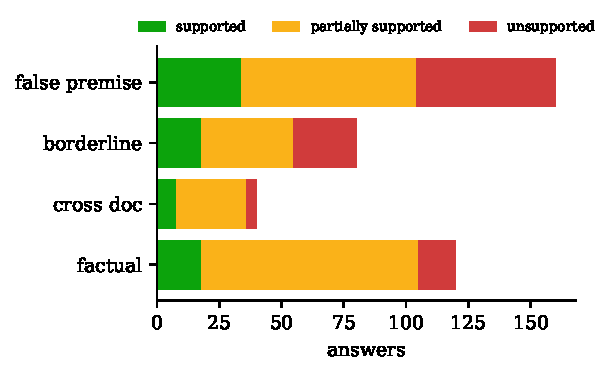
\includegraphics[width=\columnwidth]{figures/labels_by_category.pdf}}{}
\caption{Primary-judge verdicts per question category.}\label{fig:labels}
\end{figure}

\subsection{Detection}
\Cref{tab:cv} and \cref{fig:roc} summarise \CVProtocol. EpistemeGraph reaches AUROC \CVAUC{} (fold s.d.\ \CVAUCsd;
95\% CI [\CVAUCLo, \CVAUCHi]) with ECE \CVECE. The audited model's verbalised confidence reaches only \CVAUCllm{} with
ECE \CVECEllm{} ($p=\CVPllm$ against EpistemeGraph), and the detector exceeds the length confound (\CVAUClen,
$p=\CVPlen$). The text-only NLI checker given the same pooled claim evidence is close (\CVAUCtext, $p=\CVPtext$), and
the same learner on the 13 answer-level features alone is indistinguishable (\CVAUCvthree, $p=\CVPvthree$). With the
first, noisier labels the claim-set representation had improved that learner from \HaikuLabelCVAUCvthree{} to
\HaikuLabelCVAUC; with the stronger labels the gain disappears, so we do not claim it. Training on the stronger labels
changed overall AUROC only slightly (\HaikuLabelCVAUC{} to \CVAUC): two judges of different strength disagree on
different answers, and a stronger judge alone does not remove label noise. For the severe-hallucination target the
detector reaches \SevereAUC{} against \SevereLLM{} for $c_{\mathrm{LLM}}$.

\paragraph*{Robustness to the choice of judge}
On the \ConsensusN{} answers where both Claude judges agree, AUROC is \ConsensusAUC{} (versus \ConsensusLLM{} for
$c_{\mathrm{LLM}}$) and \ConsensusMatched{} of \ConsensusN{} labels are matched. Against the majority vote of all three
judges on the sample, AUROC is \MajorityAUC{} (versus \MajorityLLMAUC). Against the lenient third judge alone the
detector is at chance (\GeminiAUC) while $c_{\mathrm{LLM}}$ reaches \GeminiLLMAUC: the detector has learned the strict
``every claim supported'' definition of its training labels, and a lenient labeller ranks answers by overall
correctness, which the model's own confidence tracks better.

\TableCv

\begin{figure}[t]\centering
\IfFileExists{figures/roc_cv.pdf}{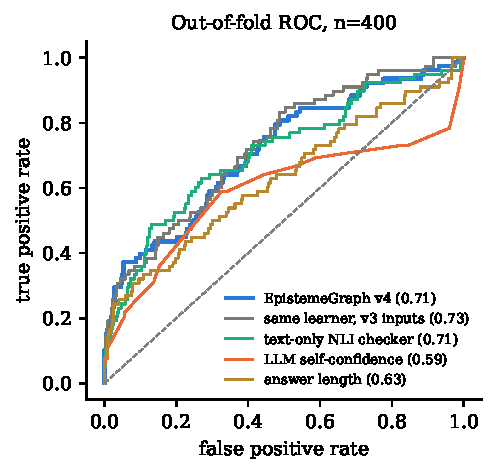
\includegraphics[width=0.95\columnwidth]{figures/roc_cv.pdf}}{}
\caption{Out-of-fold ROC curves over all labelled answers (one repetition of the repeated CV).}\label{fig:roc}
\end{figure}

\paragraph*{How many answers match the judge}
Out of fold, the detector's label (probability $\ge\frac12$) matches the primary judge on \MatchN{} of \MatchTotal{}
answers, against \MatchBase{} for always predicting ``hallucinated''; balanced accuracy is \BalAcc\%. Raw agreement is a
poor yardstick here, for two reasons. Classes are imbalanced, so a constant answer is already right \MatchBase{} times.
And agreement
between any detector and a judge is limited by how consistently the judges themselves label: two capable judges agree on
\AgreeFull\% of binary labels, and on the \ConsensusN{} answers where they agree the detector matches \ConsensusMatched.
Higher raw agreement requires cleaner labels as much as a better detector.

\paragraph*{Per category}
The categories fail differently. On \textsc{borderline} and \textsc{cross-doc} questions the verbalised confidence is
\emph{inversely} related to support (AUROC \CatBorderLLM{} and \CatCrossLLM): the model is most confident when it
invents an answer the papers do not contain or blends two papers. EpistemeGraph is strongest on \textsc{false-premise}
questions (\CatFPVfour, versus \CatFPLLM{} for $c_{\mathrm{LLM}}$); on \textsc{factual} questions the verbalised
confidence is informative (\CatFactLLM, versus \CatFactVfour). Out-of-fold scores are pooled across categories before
these AUROCs are computed.

\subsection{What the champion uses}
\Cref{tab:leaderboard} lists the tournament; with \NTrain{} training answers the neural contenders lose to boosted trees,
and the multiple-instance network is kept as the companion claim localiser. \Cref{fig:imp} and \cref{tab:claimimp}
report grouped permutation importance: after the verbalised confidence, the curvature shift $\Delta\kappa$ is the most
important answer feature, and the most important claim-level groups are NLI contradiction and entailment, out-of-corpus
rate and the grafted-edge curvature. The geometric measurements are thus used by the champion, but removing the whole
topological family does not change test AUROC significantly ($\Delta=\DeltaTopo$, $p=\PvalTopo$, \cref{tab:ablation}).
Training on the ordinal three-level verdict instead of the binary label gives AUROC \OrdAUC{} versus \BinAUC.

\TableLeaderboard
\TableAblation
\TableClaimimp

\begin{figure}[t]\centering
\IfFileExists{figures/importance_v4.pdf}{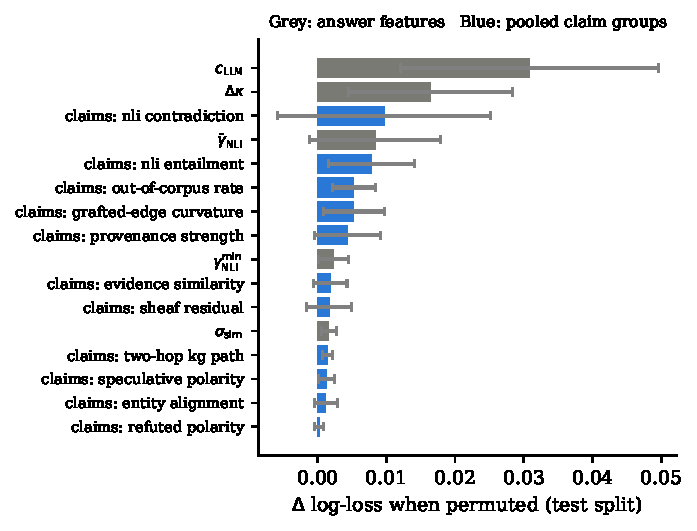
\includegraphics[width=0.95\columnwidth]{figures/importance_v4.pdf}}{}
\caption{Grouped permutation importance of the champion (increase in test log-loss, 20 repeats): answer features
(grey) and pooled claim-feature groups (blue).}\label{fig:imp}
\end{figure}

\paragraph*{The reliability pool}
On the cross-fitted training and calibration answers the KG term passes both checks ($\chi^2_1=\PoolLRTchi$,
$p=\PoolLRTp$; cross-validated log-loss \PoolCVwith{} with versus \PoolCVwithout{} without) and is therefore
\PoolKGused, but with a \emph{negative} coefficient ($b_2=\PoolBkg$, $b_1=\PoolBq$): answers whose claims touch
well-grounded KG regions are less often fully supported. We read this as the verbosity confound again, since richly
documented topics invite longer, more detailed answers. On the small test split the pooled score ranks slightly below
the pre-pool score (AUROC \TestAUC{} versus \TestAUCq), within the bootstrap interval; we report the pre-specified
procedure unchanged instead of re-selecting it on the test split.

\subsection{Calibration and decisions}
\Cref{fig:rel} shows that out-of-fold probabilities are calibrated (ECE \CVECE), whereas the verbalised confidence is
over-confident (ECE \CVECEllm). \Cref{tab:conformal} and \cref{fig:conf} give the cross-conformal trade-off over all
answers: at $\alpha=0.10$ empirical coverage is \CVCovTen\%, the system abstains on \CVAbsTen\% of answers and is
right on \CVSelTen\% of the rest; at $\alpha=0.20$ abstention falls to \CVAbsTwenty\% with selective accuracy
\CVSelTwenty\%. Over all answers, \CommittedCorrect{} of \Committed{} committed decisions at $\alpha=0.10$ are correct. On
the test split ($\alpha=\Alpha$), coverage is \Coverage\% (\CoverageSup\% supported, \CoverageHal\% hallucinated) with
abstention \AbstainRate\% and selective accuracy \SelAcc\%. On this small split the verbalised confidence happens to rank
well (AUROC \LLMAUC), in contrast to the full-data estimate (\CVAUCllm), another reason the repeated CV is primary.
Abstention is the price of a per-class guarantee with a moderately discriminative scorer and imbalanced classes.

\TableConformal
\TablePercat

\begin{figure}[t]\centering
\IfFileExists{figures/reliability_cv.pdf}{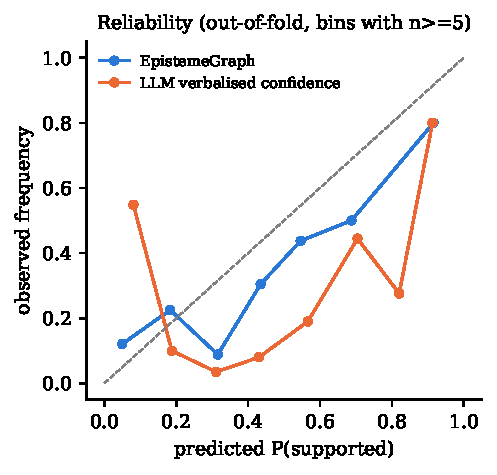
\includegraphics[width=0.9\columnwidth]{figures/reliability_cv.pdf}}{}
\caption{Reliability of out-of-fold probabilities (bins with at least five answers).}\label{fig:rel}
\end{figure}

\begin{figure}[t]\centering
\IfFileExists{figures/conformal_tradeoff.pdf}{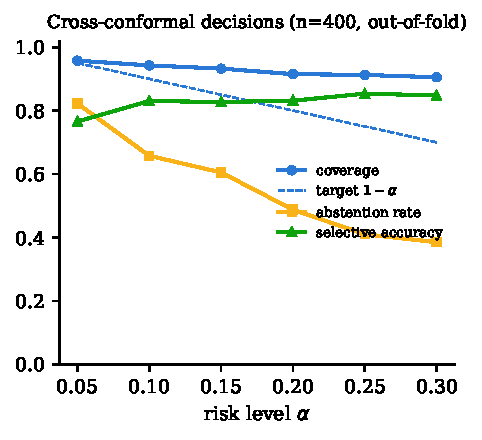
\includegraphics[width=0.9\columnwidth]{figures/conformal_tradeoff.pdf}}{}
\caption{Coverage, abstention and selective accuracy of the Mondrian cross-conformal decision as a function of $\alpha$.}\label{fig:conf}
\end{figure}

\paragraph*{Cost}
All answering, extraction, both judges and the KG audit cost \$\CostRun{} in API calls; every retraining and analysis
re-used cached artefacts at zero API cost.

% =============================================================================================
\section{Discussion and Limitations}
\label{sec:limits}

\paragraph*{Labels set the ceiling}
With $\kappa=\KappaFull$ between two LLM judges and $\kappa=\GeminiKappa$ against a judge from another family,
label noise and label \emph{definition} bound every metric in this paper; a stronger judge alone did not change the
picture. Human annotation of a stratified sample and an adjudicated label set are the natural next steps, and the
released pipeline supports both.

\paragraph*{What the geometry adds}
On this corpus, claim-level NLI against retrieved sentences and the model's own confidence carry most of the signal;
the curvature measurements are used by the champion but do not significantly beat a text checker. A larger KG (more
papers, higher recall) and richer sheaf stalks (learned restriction maps~\cite{gebhart2023knowledge}) are the natural
tests of whether geometry matters more when the reference graph is denser.

\paragraph*{Guarantees and scope}
Coverage holds per class under exchangeability, which a change of corpus, audited model, prompt or question
distribution breaks; cross-conformal calibration trades a weaker worst-case bound for stability. Three papers in one
area, one audited model, closed-book answers and \NLabelled{} labelled answers limit external validity; the full
protocol costs about two US dollars, so these limits are practical rather than methodological.

% =============================================================================================
\section{Conclusion}
\label{sec:conclusion}
EpistemeGraph treats hallucination auditing as calibrated measurement: it measures a fallible reference graph,
extracts the claim graph of an answer independently of its generation, describes every claim with evidential and
geometric instruments, and learns, rather than prescribes, how these measurements become a decision with a stated error
rate. It ranks answers far better than the audited model's own confidence (\CVAUC{} versus \CVAUCllm) and better than
a length confound (\CVAUClen). Its main lessons are methodological: audit the labels and the reference graph, control for
verbosity, report repeated cross-validation instead of one small test split, and read raw accuracy against both the
majority baseline and the agreement between judges.

\section*{Reproducibility}
Code, prompts, the benchmark, every API response, judge verdict, feature vector and trained model are released at
\url{https://github.com/Virtuoso-8051/EpistemeGraph}. All numbers in this paper are generated from these artefacts by
\texttt{scripts/analyze\_results.py} and \texttt{scripts/export\_paper\_assets.py}.

\bibliographystyle{IEEEtran}
\bibliography{references}

% =============================================================================================
\appendices
\section{Algorithms}
\label{app:alg}

\begin{algorithm}[h]
\caption{Audit of one query (inference)}
\begin{algorithmic}[1]
\Require query $q$; KG snapshot; champion $\hat p$; pool; conformal quantiles $(q_0,q_1)$
\State $a, c_{\mathrm{LLM}} \gets \textsc{Answer}(q)$
\State $G'\gets\textsc{ExtractClaims}(q,a)$ \Comment{separate call}
\State $G\gets\textsc{Retrieve}(V')$; align $V'\to V$
\State $\bm x_{\mathrm{answer}}\in\R^{13}$; $Z=\{\bm z_i\}\subset\R^{15}$; $\bm x\gets[\bm x_{\mathrm{answer}};\psi(Z)]$
\State $S_{\mathrm{query}}\gets\sigma(a\,\ell(\bm x)+b)$; $S_{\mathrm{final}}\gets$ pool$(S_{\mathrm{query}},\SKGq)$
\State $\Gamma\gets\{c:1-\hat p_c\le q_c\}$; enlarge to $\{0,1\}$ if its class is not the more probable one
\State \Return \textsc{verified} if $\Gamma=\{1\}$, \textsc{hallucinated} if $\Gamma=\{0\}$, else \textsc{abstain}
\end{algorithmic}
\end{algorithm}

\begin{algorithm}[h]
\caption{Phase 4 training}
\begin{algorithmic}[1]
\Require labelled answers $(\bm x_i,Z_i,\SKGq_i,y_i)$; risk level $\alpha$
\State split by hash(query id) into train / cal / test
\For{each family $m$}
  \State OOF$_m\gets$ outer 5-fold CV of inner 3-fold search on train
\EndFor
\State $m^\star\gets\argmin_m\mathrm{LogLoss}(\mathrm{OOF}_m)$
\State cross-fit $m^\star$ on train$\cup$cal; Platt on out-of-fold logits
\State fit pool \cref{eq:pool}; keep $b_2$ iff LRT $p<0.05$ and CV log-loss improves
\State $q_c\gets$ class-$c$ conformal quantile of out-of-fold scores
\State refit $m^\star$ on train$\cup$cal; evaluate on test; repeated CV on all data
\end{algorithmic}
\end{algorithm}

\section{Prompts and storage}
\label{app:prompts}
All prompts are versioned in the repository: KG extraction (\texttt{kg\_builder.py}), answering and claim extraction
(\texttt{llm\_interceptor.py}), benchmark generation (\texttt{scripts/generate\_benchmark.py}) and judging
(\texttt{scripts/run\_benchmark.py}). Each corpus is stored in Neo4j under its own \texttt{kg\_id} with a composite
uniqueness constraint on $(\texttt{kg\_id},\texttt{name\_key})$; evidence is replaced only by better-grounded evidence and
support counts are exact because chunk identifiers are content-addressed.

\end{document}
